\documentclass{article}
\usepackage{tikz}
\usetikzlibrary{arrows.meta,positioning,calc,shapes.geometric}
\pagestyle{empty}
\begin{document}
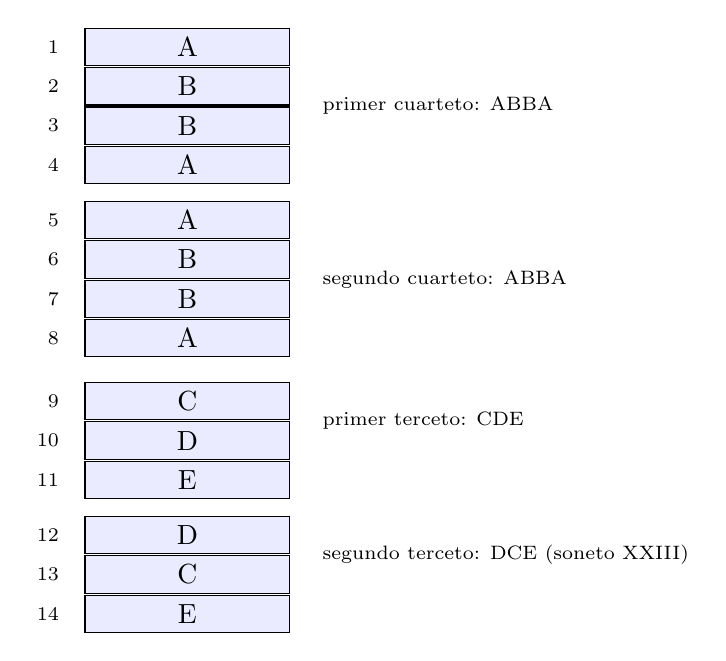
\begin{tikzpicture}

\foreach \i/\y/\r in {1/4.6/A,2/4.1/B,3/3.6/B,4/3.1/A,5/2.4/A,6/1.9/B,7/1.4/B,8/0.9/A,9/0.1/C,10/-0.4/D,11/-0.9/E,12/-1.6/D,13/-2.1/C,14/-2.6/E} {
  \node[font=\scriptsize, anchor=east] at (0.5,\y) {\i};
  \node[draw, fill=blue!8, minimum width=2.6cm, minimum height=0.4cm, anchor=west] at (0.7,\y) {\r};
}
\node[font=\scriptsize, anchor=west] at (3.6,3.85) {primer cuarteto: ABBA};
\node[font=\scriptsize, anchor=west] at (3.6,1.65) {segundo cuarteto: ABBA};
\node[font=\scriptsize, anchor=west] at (3.6,-0.15) {primer terceto: CDE};
\node[font=\scriptsize, anchor=west] at (3.6,-1.85) {segundo terceto: DCE (soneto XXIII)};

\end{tikzpicture}
\end{document}
